\documentclass[11pt,a4paper]{article}

% ------------------------------------------------
% Packages
% ------------------------------------------------
\usepackage[a4paper,margin=2cm]{geometry}
\usepackage{graphicx}
\usepackage{float}
\usepackage{titlesec}
\usepackage{enumitem}
\usepackage[hidelinks]{hyperref}
\usepackage{parskip}
\usepackage{xcolor}

\setlength{\parindent}{0pt}
\setlist[itemize]{noitemsep, topsep=0pt}


\titleformat{\section}{\large\bfseries}{}{0em}{}[\titlerule]

\begin{document}

\begin{minipage}{0.72\textwidth}
    {\LARGE \textbf{Daniel Gräf}}\\
B.Sc. Technische Informatik (Abschluss Sommer 2026) \\
Rommerskirchen, Deutschland \\
+49 1523 1094514 \quad | \quad \href{mailto:daniel.graef14@gmail.com}{daniel.graef14@gmail.com}
\end{minipage}
\hfill
\begin{minipage}{0.25\textwidth}
    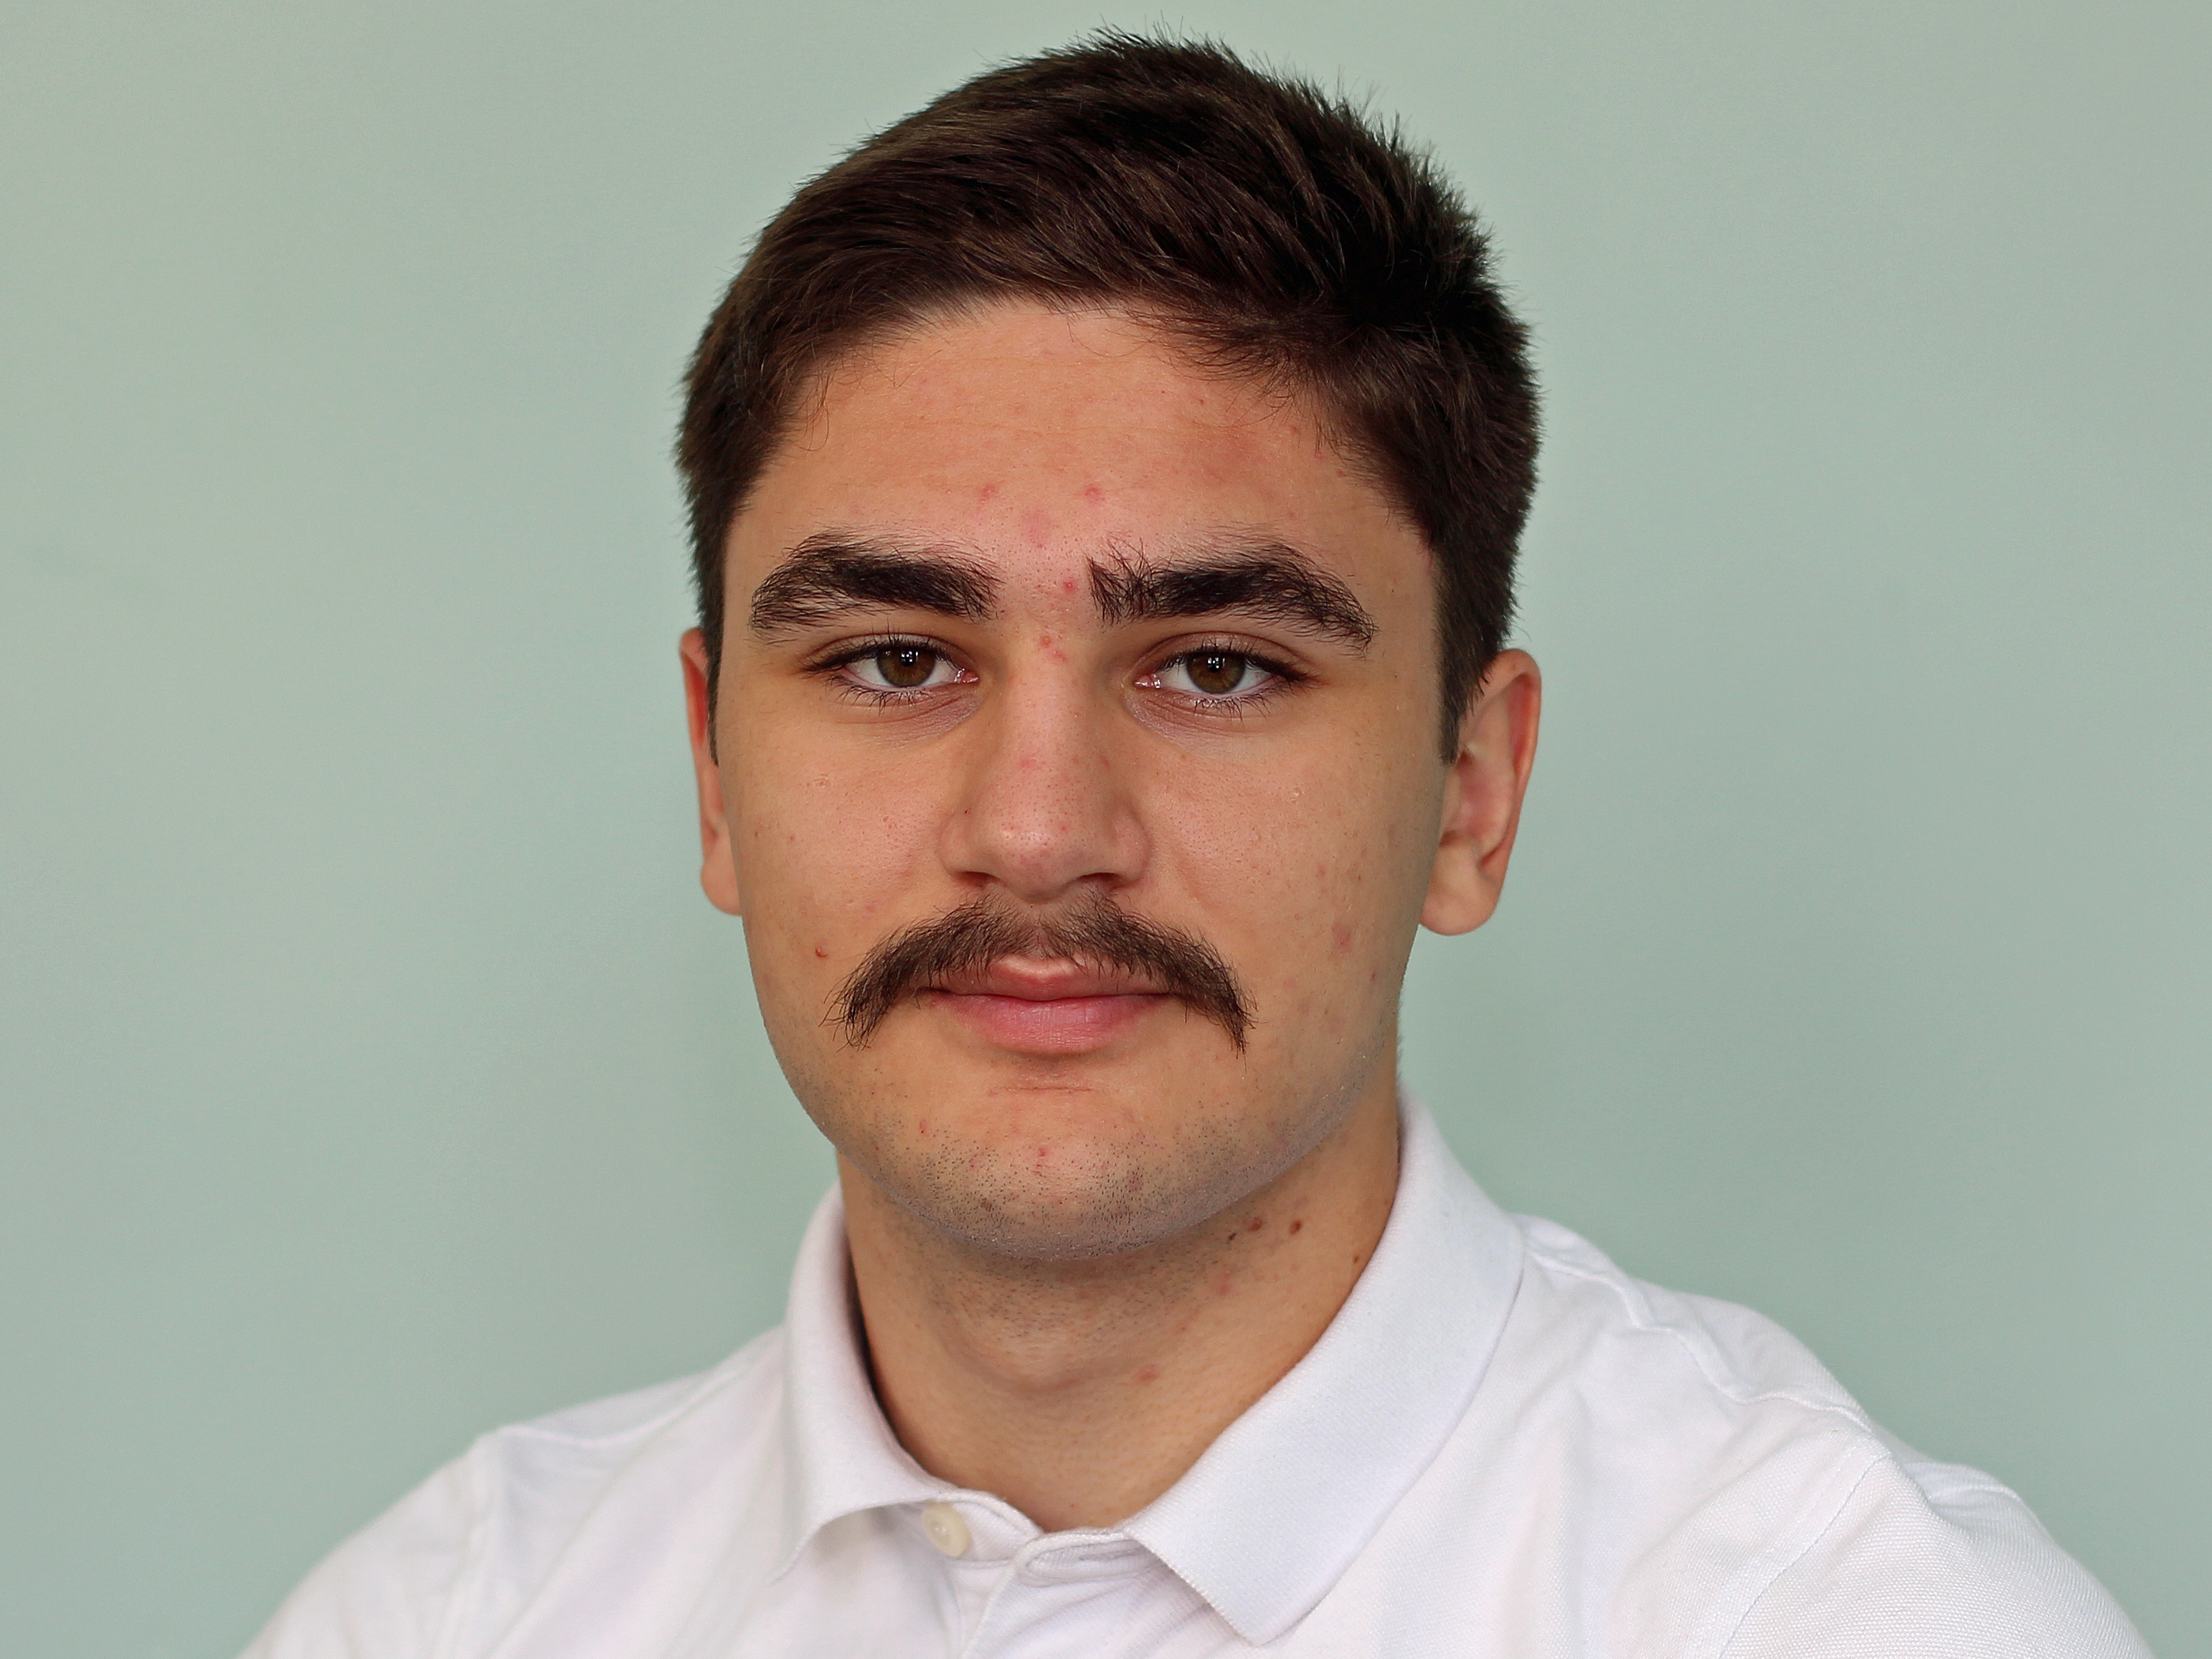
\includegraphics[width=\linewidth]{Daniel_Graef.jpg}
\end{minipage}


%================================================
\section*{Profil}
%================================================

Softwareentwickler mit sehr starker Python-Expertise und ausgeprägtem Systemverständnis.
Fokus auf Architektur, Automatisierung und der strukturierten Abbildung komplexer technischer Prozesse.
Arbeite analytisch, eigenverantwortlich und mit hoher Leistungsorientierung.

%================================================
\section*{Berufserfahrung}
%================================================

\textbf{Werkstudent – Pierburg GmbH (Rheinmetall-Konzern)} \hfill Seit 2024

\begin{itemize}[leftmargin=*]
    \item Entwicklung webbasierter Oberflächen mit \textit{optiSLang} und \textit{pyOwa}
    \item Automatisierung komplexer CAD-Simulations-Workflows
    \item Abbildung technischer Parameter und Simulationsergebnisse
          in benutzerfreundlichen Webinterfaces
    \item Reduktion der Abhängigkeit von Simulationsexperten
          durch strukturierte Parametrisierung und Ergebnisaufbereitung
\end{itemize}

%================================================
\section*{Ausbildung}
%================================================

\textbf{Technische Hochschule Köln} \hfill 2023 – 2026 \\
Bachelor Technische Informatik \\
Notenschnitt: 1,7 \\
Abschluss in verkürzter Studienzeit (6 Semester)

\begin{itemize}[leftmargin=*]
    \item Module u.a.: Softwareentwicklung (Java, C),
          Rechnerarchitektur, Netzwerktechnik, Digitaltechnik
    \item Geplanter Master: Technische Informatik (ab WS 2026)
\end{itemize}

%================================================
\section*{Technische Kompetenzen}
%================================================

\textbf{Kernkompetenzen:}
Python (Experte), Java (sehr gut), Softwarearchitektur, Systemdesign, Linux

\textbf{Machine Learning \& KI:}
Fundierte Kenntnisse in Machine Learning und KI-Anwendungen,
praktische Erfahrung mit TensorFlow, PyTorch, NumPy (Python-basiert)

\textbf{Weitere Technologien:}
Kotlin, SQL, React, Docker, Kubernetes (Grundlagen), C (Grundlagen)

%================================================
\section*{Ausgewählte Projekte}
%================================================

\textbf{PDF-Automatisierungstools (Industrieeinsatz bei INEOS)}
\begin{itemize}[leftmargin=*]
    \item Entwicklung mehrerer Python-Tools zur strukturierten Analyse
          technischer PDF-Dokumente
    \item Produktiver Einsatz zur signifikanten Reduktion manueller Recherchearbeit
    \item Eigenständige Architektur, Implementierung und Weiterentwicklung
\end{itemize}

\textbf{Autonomes Rover-System}
\begin{itemize}[leftmargin=*]
    \item Vollständige Hard- und Softwareplanung eines sensorbasierten Systems
    \item Entwicklung eines Simulations- und Visualisierungstools
          zur Validierung von Navigationsalgorithmen
    \item Integration von LiDAR-, Ultraschall- und Gyrosensorik
\end{itemize}

\textbf{Systementwurfspraktikum – Teamleitung}
\begin{itemize}[leftmargin=*]
    \item Leitung eines 5-köpfigen Entwicklerteams
    \item Konzeption und Umsetzung einer Raumfindungs-App für die TH Köln
    \item Architekturdefinition, Aufgabenstrukturierung und Implementierung
\end{itemize}

%================================================
\section*{Weitere technische Projekte}
%================================================

\textbf{HomeAssistant-System (Eigenentwicklung)}
\begin{itemize}[leftmargin=*]
    \item Aufbau und Integration eines vollautomatisierten Smart-Home-Systems
    \item KNX/EIB-Anbindung zur Steuerung von Temperatur, Fensterstatus
          und Warmwasser
    \item Integration von Kalender- und Ereignislogik zur Alltagsautomatisierung
\end{itemize}

%================================================
\section*{Persönliche Leistungsnachweise}
%================================================

\textbf{Schach}
\begin{itemize}[leftmargin=*]
    \item Elo 2200 auf Chess.com (Top 0,5\% weltweit)
    \item Schachkreismeister in der Jugend
\end{itemize}

\textbf{Sportlicher Hintergrund}
\begin{itemize}[leftmargin=*]
    \item 10 Jahre leistungsorientierter Fußball, Kreisauswahl
    \item In mehreren Mannschaften nach kurzer Zeit zum Kapitän gewählt
    \item Aktuell: Thaiboxen, Laufen, Schwimmen, Radfahren, Wandern, Skifahren
\end{itemize}

\end{document}